\section{Music Generation}

\subsection{Lakh MIDI Dataset}
The dataset used in this project is part of the Lakh MIDI Dataset \cite{lakh}. The full dataset is composed of 176 thousand MIDI files divided by artist.
I selected two subsets of files from the Lakh MIDI Dataset:
\begin{enumerate}
	\item 120 MIDI files are randomly and equally divided into three genres of different artist and all containing the piano instrument;
	\label{dataset1}
	\item 120 MIDI files of only one genre of different artists and all containing the piano instrument;
	\label{dataset2}
	\item 40 MIDI files are randomly and equally divided into three genres of different artist and all containing the piano instrument (this is a subset of the initial one);
	\label{dataset3}
\end{enumerate}
The third dataset is a subset of the dataset n.1 and it was used for the model selection.
The total number of MIDI files used in this project is 200. The 200 MIDI files are divided in three genres of different artist and all containing the piano instrument: Metal, Pop Rock and Rock.
For the initial model choice, a subset of this 200 MIDI files has been used: 30 MIDI files for the training, 6 for the validation and 3 for the test, all chosen in a randomly and equally way between the 3 genres.
From these dataset 3 models were trained, tested and compared:
\begin{itemize}
	\item A model based on the full dataset n.1;
	\item A model based on the piano instrument MIDI part of the dataset n.1;
	\item A model based on the full dataset n.2;
\end{itemize}
Each model was trained on 85\% of the dataset, validated and tested on the remaining 15\%.
The MIDI representation is a technical standard for controlling and synchronizing digital instrument. 
This is a really interesting representation because through the use of compatible libraries it is possible to extract the instruments used in the songs. 

\begin{comment}
	Parlare del dataset
	100 canzoni per il training e 20 per validation e test
	Parlare dei file MIDI
	Parlare che la scelta del modello è stato fatto su un subset delle 100
	3 generi musicali, n strumenti
	3 modelli quelli finali: 1 su 3 generi con tutti gli strumenti, 1 su 1 solo genere con tutti gli strumenti e 1 su 3 generi con soltanto il basso elettrico
\end{comment}

\subsection{Transformer model: vanilla and XL}
\label{sec:transformer}
The architecture used in this project is the compressive transformers \cite{raecompressive2019}. This architecture is an expansion of the Transformer XL \cite{tranformerxl} and also of the vanilla architecture \cite{AIAYN}. The main component of this two architectures are the self-attention and the introduction of more memory in the Transformer XL. The vanilla architecture has an encoder-decoder design as you can see in figure \ref{fig:vanilla_model}. The general data flow is, given a sequence of tokens x they are mapped in a continuous representation z. The decoder takes as input one element of z at a time with the additional input of the previous output generated by itself (the model is auto-regressive).
\begin{figure}[H]
	\begin{center}
		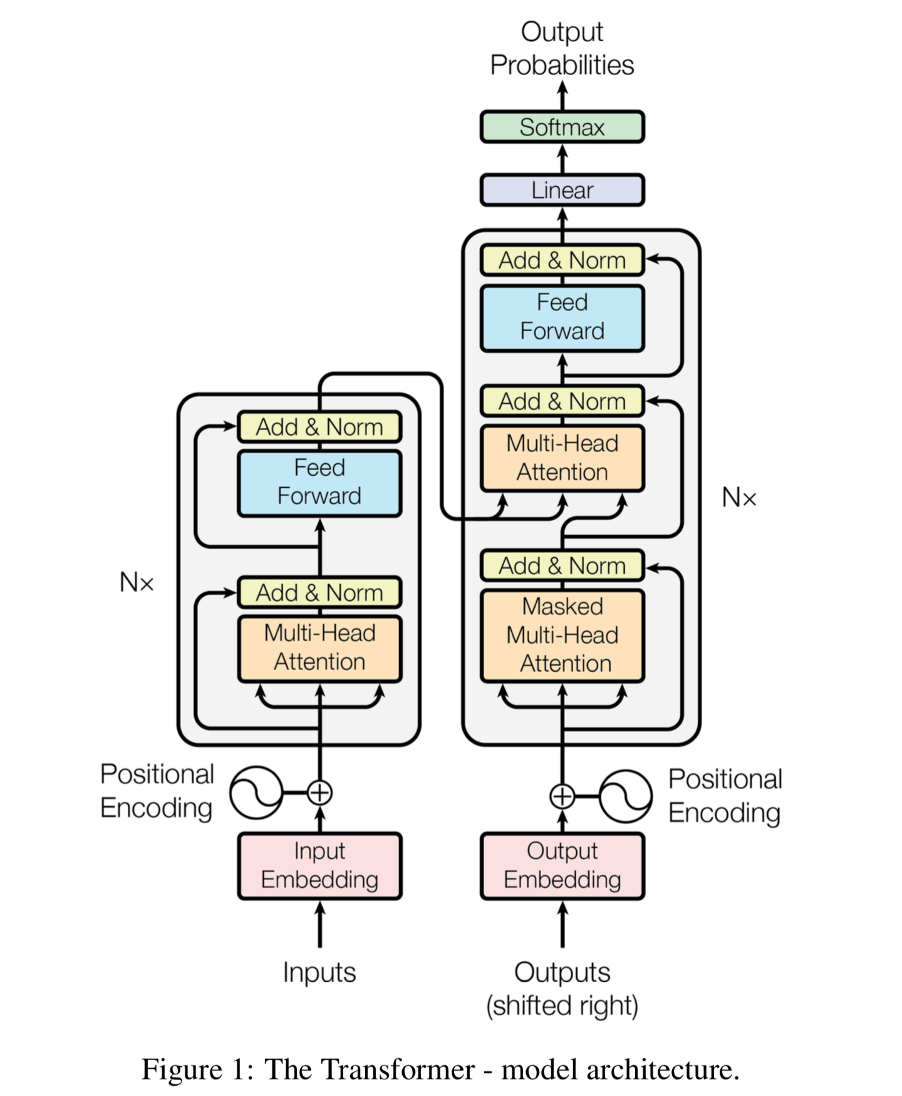
\includegraphics[width=0.4\linewidth]{img/tranformer_architecture.png}
	\end{center}
	\caption{Model architecture of the vanilla transformer.}
	\label{fig:vanilla_model}
\end{figure} 

\begin{wrapfigure}[19]{l}{0.40\textwidth}
	\begin{center}
	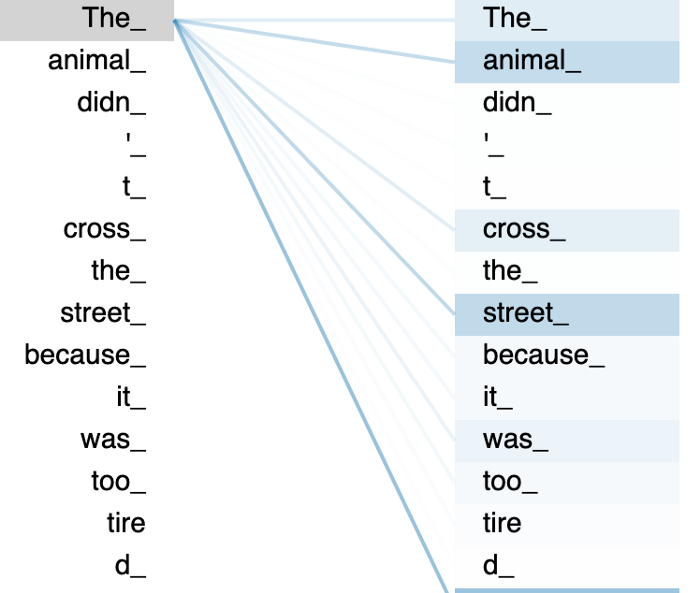
\includegraphics[width=1\linewidth]{img/nl_seq.png}
	\end{center}
	\caption{Encoding of the word "The" and measure of the attention paid to other token in the sequence.}
	\label{fig:nl_seq}
\end{wrapfigure}
\subsubsection{Vanilla Self-Attention}
The main idea of the self-attention \cite{AIAYN} is to learn and describe the relationship between tokens in a sequence. This could be done in different ways (e.g. using the cosine similarity or the scaled dot-product attention equation \ref{eq:self-attention}). But, the main observation is to have an attention function that given a vector query Q, the matrices of keys K and values V it computes as output the relationship between them. The input Q and K have dimension $d^{k}$.
\begin{equation}
	Attention(Q,K,V) = softmax(\frac{Q*K^{T}}{\sqrt{d^{k}}})*V
	\label{eq:self-attention}
\end{equation} 
\newline
The self-attention can be explained in a clear way using a natural language sequence. As you can see in figure \ref{fig:nl_seq}, when we encode the first token of the sequence (this happens also for the other token) we can see clearly on which other words the token "The" is focusing. This happens also for the decoding part (in which we had to pay attention not to look at subsequent positions).

\subsubsection{Transformer XL new techniques}

Two important techniques were introduced by the Transformer XL to overcome the vanilla shortcomings:
\begin{itemize}
	\item \textit{Recurrence Mechanism}: as said in \S\ref{sec:memory_compression}, this technique enables long-term dependencies by using information from previous segments. This is done conditioning the K and the V value of the current segment with the previously hidden state sequence produced by the previous segment concatenated with the earlier hidden state sequence produced by the current segment.
	To have a better understanding of the practical computation, in formulas \ref{eq:Recurrence_Mechanism1}, \ref{eq:Recurrence_Mechanism2} and \ref{eq:Recurrence_Mechanism3} you can find the mathematical explanation given by the authors of the paper \cite{tranformerxl}.
	\begin{gather} 
	\text{Let } s_{\tau} = [x_{\tau, 1}, ... , x_{\tau, L}] \notag \\
	\text{ be the } \tau \text{-th segment of length L } h_{\tau}^{n} \in \Re^{L\times d}, \notag \\
	\text{where n = number of hidden layers and d = hidden dimension} \notag\\
	\text{Then for segment}  s_{\tau+1}\text{, hidden state of n-th hidden layer is given by:} \notag\\
	\widetilde{h}_{\tau+1}^{n-1} = [SG(h_{\tau}^{n-1}) \circ h_{\tau+1}^{n-1}] \label{eq:Recurrence_Mechanism1}\\
	q_{\tau+1}^{n}, k_{\tau+1}^{n}, v_{\tau+1}^{n} = h_{\tau+1}^{n-1} \cdot W_{q}^{\mathsf{T}}, \widetilde{h}_{\tau+1}^{n-1} \cdot W_{k}^{\mathsf{T}}, \widetilde{h}_{\tau+1}^{n-1} \cdot W_{v}^{\mathsf{T}} \label{eq:Recurrence_Mechanism2} \\
	h_{\tau+1}^{n}=\text { Transformer-Layer }\left(q_{\tau+1}^{n}, k_{\tau+1}^{n}, v_{\tau-1}^{n}\right) \label{eq:Recurrence_Mechanism3} \\
	\text{where } \mathrm{SG}(\cdot) \text{ is stop gradient,} \notag \\
	\left[h_{u} \circ h_{v}\right] \text{ is concatenation operation along length dimension} \notag \\
	\text{ and W denotes learnable model parameters} \notag
	\end{gather} 
	
	\item \textit{Relative Positional Encoding}: the recurrence mechanism introduce a new problem in the positional encoding of the transformer, now the current sequence and the previous one will have the same positional encoding. For this reason, a relative position encoding was introduced to compute correctly the self attention of the current segment. To have a better understanding of the mathematical process, in formulas  \ref{eq:Relative_Positional_Encoding1}, \ref{eq:Relative_Positional_Encoding2} and \ref{eq:Relative_Positional_Encoding3} you can find the explanation given by the authors of the paper \cite{tranformerxl}.
	
	In the vanilla Transformer, the attention score between query $q_{i}$ and key $k_{j}$ within the same segment is:
	\begin{align}
	\label{eq:Relative_Positional_Encoding1}
	\mathbf{A}_{i, j}^{\mathrm{abs}} &=\operatorname{query}\left(x_{i}\right) \cdot \operatorname{key}\left(x_{j}\right) \notag\\
	&=\left[\mathbf{W}_{q}\left(\mathbf{E}_{x_{i}}+\mathbf{U}_{i}\right)\right]^{T}\left[\mathbf{W}_{k}\left(\mathbf{E}_{x_{j}}+\mathbf{U}_{j}\right)\right] \\
	&=\left(\mathbf{E}_{x_{i}}+\mathbf{U}_{i}\right)^{T} \mathbf{W}_{q}^{T} \mathbf{W}_{k}\left(\mathbf{E}_{x_{j}}+\mathbf{U}_{j}\right) \notag
	\end{align}
	After simplification:
	\begin{align}
	\label{eq:Relative_Positional_Encoding2}
	\mathbf{A}_{i, j}^{\mathrm{abs}} =\underbrace{\mathbf{E}_{x_{i}}^{\top} \mathbf{W}_{q}^{\top} \mathbf{W}_{k} \mathbf{E}_{x_{j}}}_{(\boldsymbol{a})}+\underbrace{\mathbf{E}_{x_{i}}^{\top} \mathbf{W}_{q}^{\top} \mathbf{W}_{k} \mathbf{U}_{j}}_{(b)} \notag\\
	+\underbrace{\mathbf{U}_{i}^{\top} \mathbf{W}_{q}^{\top} \mathbf{W}_{k} \mathbf{E}_{x_{j}}}_{(c)}+\underbrace{\mathbf{U}_{i}^{\top} \mathbf{W}_{q}^{\top} \mathbf{W}_{k} \mathbf{U}_{j}}_{(d)}
	\end{align}
	Authors re-parameterised the 4 terms as:
	\begin{align}
	\label{eq:Relative_Positional_Encoding3}
	\mathbf{A}_{i, j}^{\mathrm{rel}} &=\underbrace{\mathbf{E}_{x_{i}}^{\mathrm{T}} \mathbf{W}_{q}^{\top} \mathbf{W}_{k, E} \mathbf{E}_{x_{j}}}_{(a)}+\underbrace{\mathbf{E}_{x_{i}}^{\top} \mathbf{W}_{q}^{\top} \mathbf{W}_{k, R} \mathbf{R}_{i-j}}_{(b)} \notag\\
	&+\underbrace{u^{\top} \mathbf{W}_{k, E} \mathbf{E}_{x_{j}}}_{(c)}+\underbrace{v^{\top} \mathbf{W}_{k, R} \mathbf{R}_{i-j}}_{(d)}
	\end{align}
	\begin{itemize}
		\item Replace all $U_{j}$ with $R_{i-j}$ as the relative distance matters for where to attend;
		\item Replace the query $\mathbf{U}_{i}^{\top} \mathbf{W}_{q}^{\top}$ with $u \in \mathbb{R}^{d}$ in term $(c)$.
		$\mathbf{U}_{i}^{\top} \mathbf{W}_{q}^{\top}$ is the absolute positional encoding for the query. As it is the same for all query positions (we only care about relative key position) we use $u$. Similarly, we replace term $(d)$ with $v$;
		\item Separate the two-weight matrices $W_{k, E}$ and $W_{k, R}$ for producing content-based key vectors and location-based key vectors respectively.
	\end{itemize}
	
	
	
\end{itemize}

\subsection{Compressive Transformers architecture}

The compressive transformer architecture is based on the Transformer XL architecture \cite{tranformerxl} with the addition of compressed memory. As stated in \S\ref{sec:transformer} the core structure is the same for all the three models (vanilla, XL and compressed). Now, we can understand why and how the memory compression was added and which compression functions and loss were used in the paper \cite{raecompressive2019}.

\subsubsection{Memory compression}
\label{sec:memory_compression}
In the Transformer XL \cite{tranformerxl} was introduced the recurrence mechanism. The goal of the recurrence mechanism is to overcome the vanilla shortcomings enabling long-term dependencies by using information from previous segments. This requires the addition of memory to store the information of the past segments. For obvious reasons, the memory cannot be of infinite size and in this way, we could lose some important information deriving from previous segments. At this point, we could introduce the memory compression to help us store as much information as we can. In particular, through the compressed memory as you can see in figure \ref{fig:comprssed_memory}, we can achieve a longer temporal range. Suppose that our Transformer XL has $l$ layers, $m$ as memory size and $n$ as sequence length, the maximum temporal range is $l*m$ with an attention cost of $\O(n^2 + n*m)$. Suppose having the transformer XL but with memory m divided in $m_{s}$ as standard memory and $m_{cm}$ as compressed memory, and c as the rate of compression, the maximum temporal range is of $l*(m_{s} + c*m_{cm})$ with an attention cost of $\O(n^2 + n*(mm_{s} + m_{cm}))$. 


\begin{figure}[H]
	\begin{center}
		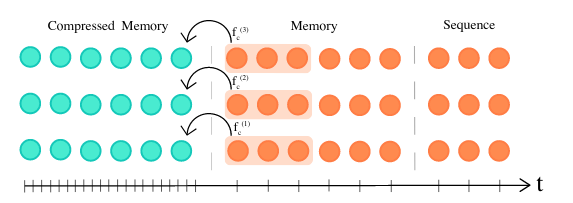
\includegraphics[width=0.7\linewidth]{img/compressed_memory.png}
	\end{center}
	\caption{Example of compressed memory in a transformer with 3 layer, a sequence length of 3, a memory size of 6, a compressed memory size of 6 and rate of compression of 3.}
	\label{fig:comprssed_memory}
\end{figure}


\subsubsection{Compression functions and loss}
The compression function could be chosen between a wide range of function, in the original paper of the compressive transformers \cite{raecompressive2019} four different functions were considered:
\begin{itemize}
	\item max/mean pooling (kernel and stride set to c);
	\item 1D convolution (kernel and stride set to c, take into consideration only its layer information);
	\item dilated convolutions (reducing the space taking also the spatial correlation between information);
	\item most-used (where only most used memory was preserved).
\end{itemize}
In my opinion, the authors of the paper \cite{raecompressive2019} decided to explore this compression function because they are at the same time simple to use and fast to compute.

The loss function used for the Transformer task objective is the cross-entropy loss.
The most performing loss for the compression network was the attention-reconstruction loss (algorithm \ref{alg:Attention_Reconstruction_Loss}) because our goal is to reconstruct the original memory. Also, all the information that are no longer attended can be discarded.

\begin{algorithm}[H]
	\caption{Attention-Reconstruction Loss.}
	\label{alg:Attention_Reconstruction_Loss}
	\begin{algorithmic}[1]
		\State $L^{attn} \gets 0$
		\For {layer i = 1, 2,..., l} 
		\State $h^{(i)} \gets$ stop\_gradient$(h^{(i)})$
		\State $old\_mem^{(i)} \gets$ stop\_gradient$(old\_mem^{(i)})$
		\State Q, K, V $\gets$ stop\_gradient(attenstion params at layer i)
		\State def attn(h,m) $\gets$ $\sigma$((h$\cdot$Q)$\cdot$(m$\cdot$K))$\cdot$(m$\cdot$V)
		\State $new\_cm^{(i)} \gets$ $f_{c}^{i}(old\_mem^{(i)})$
		\State $L^{attn} \gets L^{attn}$ + $\parallel$attn$(h^{(i)},old\_mem^{(i)})$ - attn$(h^{(i)},new\_cm^{(i)})$$\parallel_{2}$
		\EndFor
	\end{algorithmic}
\end{algorithm}
\subsection{Experiments}
The architecture is based on the implementation of Phil Wang \cite{compressive_library} of the compressive transformers. Now I am going to describe the exact architecture used for all three datasets. The input consists of a vector of 64 notes and chords. Then, there are the encoder and the decoder, for a total of 6 residual layers. All the models were trained with Adam PyTorch Optimizer. Different configurations of the architecture were validated, the first important parameter searched was the sequence length. Three sizes were taken into consideration: 32, 64 and 128. After some considerations about the pros and cons of each configuration, like information understanding and correlation, costs and time for training and probability of overfitting or underfitting, I chose to use 64 as sequence length. Also, the regularization is important in this kind of tasks with models with a large number of parameter. For this reason, I tried two types of models, one without regularization and one with 0.1 of dropout parameter. 


\subsection{Training}
\label{training}
The training was computed on Google Colab (with Nvidia k80, T4 and P100 gpu). Each model was trained at least for 100 epochs. Each epoch had a time to compute in the range of 200 to 500 seconds for dataset \ref{dataset1} and \ref{dataset2} and of in the range of 60 to 80 seconds for dataset \ref{dataset3}.
A summary of the execution results is available in the table \ref{tab:training_value}.
Interesting behaviors can also be observed in figures \ref{fig:d1}, \ref{fig:piano}, \ref{fig:d2} and \ref{fig:d3}.
First of all, in all the plots are visible the positive effects of the regularization (only the dropout regularization was tested because it was the only type available in the library). As expected from the theory, the models trained with dropout regularizer decreases the variance with respect to models without.
Also, the models trained with dataset \ref{dataset1} and \ref{dataset2} shows that a large dataset decreases the overfitting risk. Following that, it is possible to observe that the models trained with piano \ref{dataset1} and \ref{dataset3} show overfitting in less than 50 epoch.
In conclusion, in figure \ref{fig:d1} and \ref{fig:d2} it is possible to see that the adam optimizer changed the approached local minima and I think that this is due to the regularization. 
\begin{center}
	\small\addtolength{\tabcolsep}{-3pt}
	\begin{table}[h!]
		\centering
		\begin{tabular}{|c|c|c|c|c|c|c|c|}
			\hline
			\textbf{Dataset}& \textbf{Epoch} & \textbf{Best epoch} & \textbf{Dropout} & \textbf{Error TR} & \textbf{Error VL}\\ \hline
			\ref{dataset1} & 700 & 435 & 0 & 2.6694 & 3.5057 \\			\ref{dataset1} & 671 & 570 & 0.1 & 2.5349 & 3.4274 \\		 
			Piano \ref{dataset1} & 104 & 40 & 0 & 2.5028 & 4.1092 \\			
			Piano \ref{dataset1} & 148 & 105 & 0.1 & 2.6281 & 4.0401 \\			\ref{dataset2} & 228 & 135 & 0 & 2.7016 & 3.2504 \\			\ref{dataset2} & 525 & 400 & 0.1 & 2.7504 & 3.0382 \\			\ref{dataset3} & 255 & 30 & 0 & 2.3218 & 4.3809 \\			\ref{dataset3} & 187 & 25 & 0.1 & 2.5188 & 4.3612 \\
			\hline
		\end{tabular}
		\caption{Best epoch training and validation error value.}
		\label{tab:training_value}
	\end{table}
\end{center}

\begin{figure}[H]
	\centering
	\begin{minipage}[t]{0.5\linewidth}
		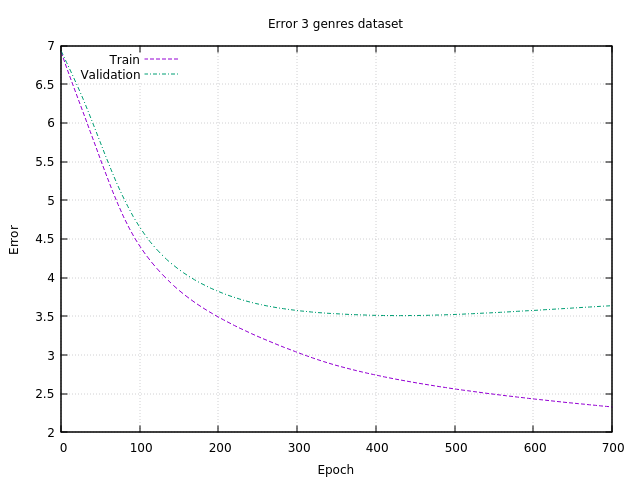
\includegraphics[width=\linewidth]{img/Plot/full/plot_full_64_0_drop.png}
		\subcaption{Without dropout.}
	\end{minipage}%
	\begin{minipage}[t]{0.5\linewidth}
		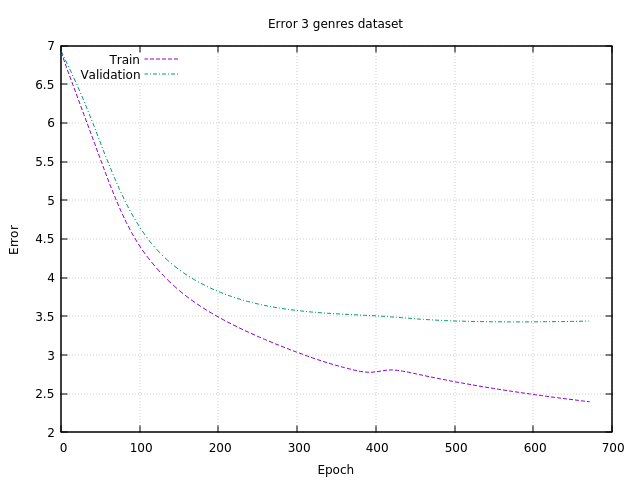
\includegraphics[width=\linewidth]{img/Plot/full/plot_full_64_0.1_drop.png}
		\subcaption{With 0.1 of dropout.}
	\end{minipage}
	\caption{Learning curves with dataset \ref{dataset1}.}
	\label{fig:d1}
\end{figure}
\begin{figure}[H]
	\centering
	\begin{minipage}[t]{0.5\linewidth}
		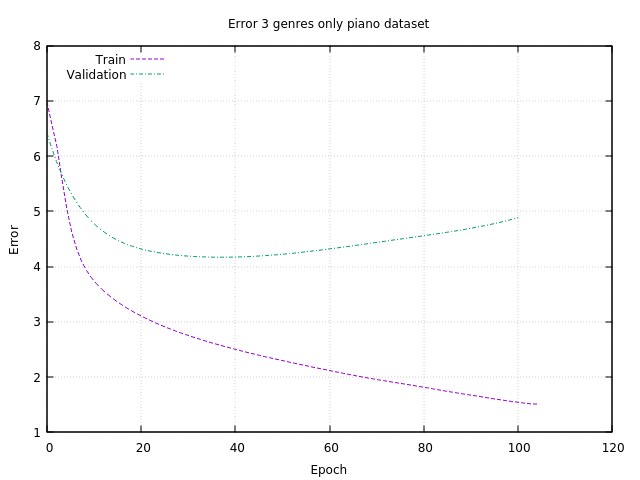
\includegraphics[width=\linewidth]{img/Plot/piano/plot_piano_64_0_drop.png}
		\subcaption{Without dropout.}
	\end{minipage}%
	\begin{minipage}[t]{0.5\linewidth}
		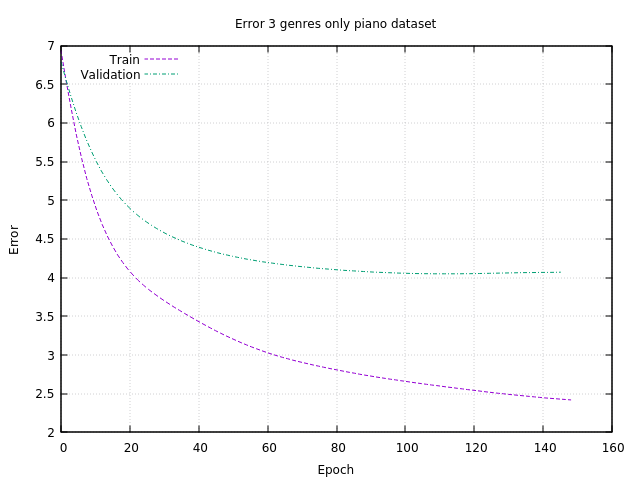
\includegraphics[width=\linewidth]{img/Plot/piano/plot_piano_64_0.1_drop.png}
		\subcaption{With 0.1 of dropout.}
	\end{minipage}
	\caption{Learning curves with only notes and chords containing piano instrument of dataset \ref{dataset1}.}
	\label{fig:piano}
\end{figure}
\begin{figure}[H]
	\centering
	\begin{minipage}[t]{0.5\linewidth}
		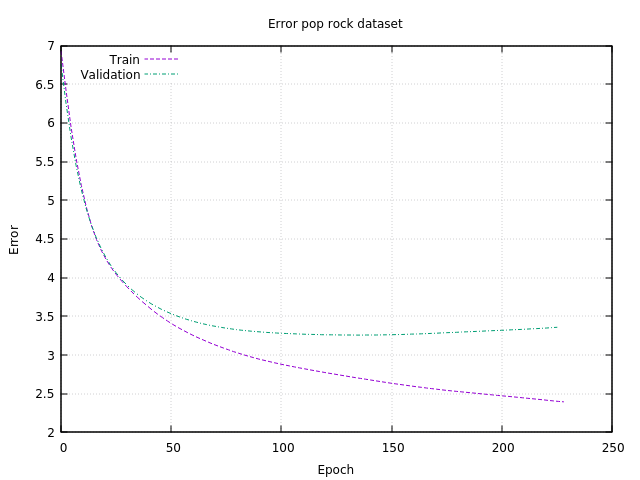
\includegraphics[width=\linewidth]{img/Plot/pop_rock/plot_pop_rock_64_0_drop.png}
		\subcaption{Without dropout.}
	\end{minipage}%
	\begin{minipage}[t]{0.5\linewidth}
		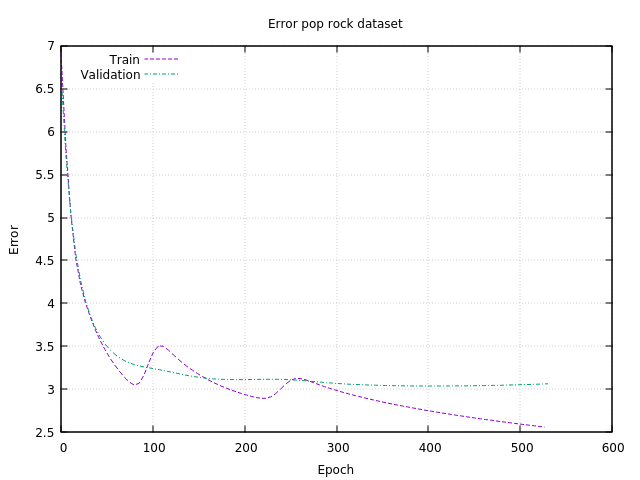
\includegraphics[width=\linewidth]{img/Plot/pop_rock/plot_pop_rock_64_0.1_drop.png}
		\subcaption{With 0.1 of dropout.}
	\end{minipage}
	\caption{Learning curves with dataset \ref{dataset2}.}
	\label{fig:d2}
\end{figure}
\begin{figure}[H]
	\centering
	\begin{minipage}[t]{0.5\linewidth}
		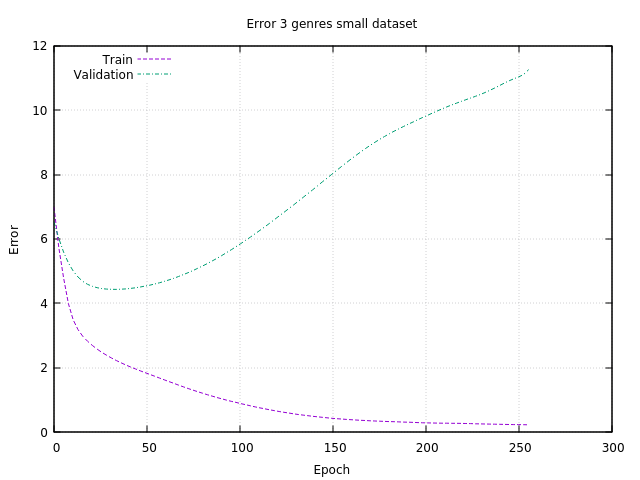
\includegraphics[width=\linewidth]{img/Plot/small/plot_small_64_0_drop.png}
		\subcaption{Without dropout.}
	\end{minipage}%
	\begin{minipage}[t]{0.5\linewidth}
		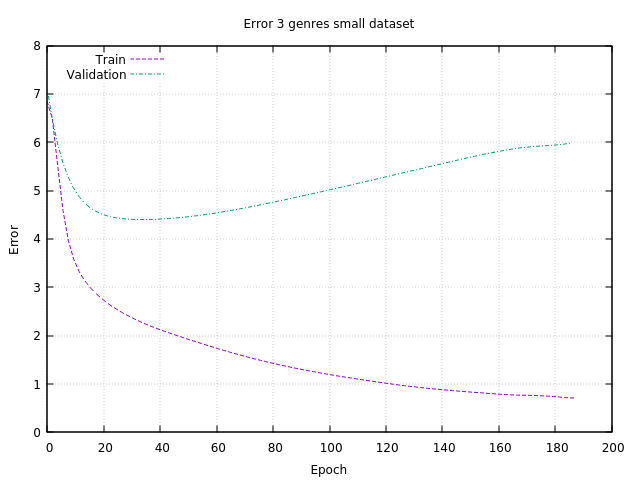
\includegraphics[width=\linewidth]{img/Plot/small/plot_small_64_0.1_drop.png}
		\subcaption{With 0.1 of dropout.}
	\end{minipage}
	\caption{Learning curves with dataset \ref{dataset3}.}
	\label{fig:d3}
\end{figure}

\subsection{Model comparison}
All the models presented in \S \ref{training} were tested on a dataset of 8 songs of 3 different genres and all containing the instrument piano.
The results are presented in table \ref{tab:test_value}:

\begin{center}
	\small\addtolength{\tabcolsep}{-3pt}
	\begin{table}[h!]
		\centering
		\begin{tabular}{|c|c|c|c|c|c|c|c|}
			\hline
			\textbf{Dataset}& \textbf{Dropout} & \textbf{Error TR} & \textbf{Error VL} & \textbf{Error TS}\\ \hline
			\ref{dataset1} &  0 & 2.6694 & 3.5057 & 4.3238 \\
			\ref{dataset1} &  0.1 & 2.5349 & 3.4274 & 4.2746 \\		 
			Piano \ref{dataset1} & 0 & 2.5028 & 4.1092 & 4.8609 \\			
			Piano \ref{dataset1} & 0.1 & 2.6281 & 4.0401 & 4.7762 \\	
			\ref{dataset2} & 0 & 2.7016 & 3.2504 & 4.4305 \\	
			\ref{dataset2} & 0.1 & 2.7504 & 3.0382 & 4.1874 \\
			\ref{dataset3} & 0 & 2.3218 & 4.3809 & 5.8341 \\
			\ref{dataset3} & 0.1 & 2.5188 & 4.3612 & 5.4717\\
			\hline
		\end{tabular}
		\caption{Best epoch training and validation error value.}
		\label{tab:test_value}
	\end{table}
\end{center}




Using as baseline the models trained on full dataset \ref{dataset1}, It is possible to do some comparisons. First, from table \ref{tab:test_value}, it is possible to observe that the model trained only on Piano instrument, does not perform as the others. From this, I can conclude that it is better to consider possibly all the instruments used at each time. Surprisingly, the model trained only on one genre performed better than the baseline, I think that it is due to the similarity of the three chosen genres. Finally, the model trained on the small dataset obtained the worst value but it was presumably due to the higher probability of overfitting. In conclusion, the overall error on the training set is higher with respect to the state of the art result and I will discuss some improvement in the \S \ref{OAFMG}.
\begin{comment}

\textbf{testare i modelli sul test set e verificare come si comportano dopodichè trarre le conclusioni tra cui:
Il modello con un solo genere, generalizza bene quello con 3 generi?
Il modello con un solo strumento, generalizza bene gli altri strumenti?}
\end{comment}